% This is "sig-alternate.tex" V2.0 May 2012
% This file should be compiled with V2.5 of "sig-alternate.cls" May 2012

\documentclass{sig-alternate}
\usepackage{epstopdf}
\usepackage{booktabs}
\usepackage{color, colortbl}
\usepackage{amsmath}
\usepackage{tikz}
\usetikzlibrary{arrows}

\newtheorem{problem}{Problem}
\newtheorem{definition}{Definition}
\newtheorem{pdef}{Problem Definition}
\newtheorem{theorem}{Theorem}
\newtheorem{example}{Example}
\newtheorem{obser}{{Observation}}
\newtheorem{lemma}{{Lemma}}

\DeclareMathOperator*{\argmin}{arg\,min}
\DeclareMathOperator*{\argmax}{arg\,max}

% insert graph
%\renewcommand\textfraction{}
% emphasize,terms
\newcommand{\term}[1]{{\tt#1}}
\newcommand{\Red}[1]{\textcolor[rgb]{1.00,0.00,0.00}{#1}}
\newcommand{\Blue}[1]{\textcolor[rgb]{0.00,1.00,0.00}{#1}}
\newcommand{\Green}[1]{\textcolor[rgb]{0.00,0.00,1.00}{#1}}
\newcommand{\xch}[1]{\Blue{#1}}
\newcommand{\yh}[1]{\Red{#1}}
\newcommand{\nop}[1]{}

\begin{document}

%\title{Implicit Relation Inferring Using Knowledge Graph}
\title{From hyperlinks to semantic links}
\subtitle{A Probabilistic Approach}

%\numberofauthors{8}

%\author{
% 1st. author
%\alignauthor
%Ben Trovato\titlenote{Dr.~Trovato insisted his name be first.}\\
%       \affaddr{Institute for Clarity in Documentation}\\
%       \affaddr{1932 Wallamaloo Lane}\\
%       \affaddr{Wallamaloo, New Zealand}\\
%       \email{trovato@corporation.com}


\maketitle
\begin{abstract}
In this paper, we propose an approach for detectiing the implicit relations between 2 entities.
\end{abstract}

%\keywords{ACM proceedings, \LaTeX, text tagging}

\section{Introduction}


\section{Related Works}
%improves: incrementally training the entity-concepts so that it can model time varying attributes.(phone,manufacturer,company)--after2007-->(smartphone,manufacturer,company)




\subsection{Link entities to Database}

Linking entities to database, especially to Wikipedia, has been widely studied. Entity linking to Wikipedia~\cite{milne2008learning,mihalcea2007wikify,han2011collective} exploit Wikipedia as thesaurus and link web documents to it.
In our work, instead of linking entities to the correspond one in KB, we extract the target entity~\cite{dalvi2011automatic} and explain the semantic relation of the entity towards target entity.

%perform NER~\cite{•} in the document to link the entities. 

\subsection{Relation Discovery}
Recently, different efforts are devoted to relation Discovery~\cite{fang2011rex,shahaf2010connecting,luo2007answering} are studied on graph based approaches.
In our work, we focus on semantic relations extracted from knowledge bases to link entities with a probability.
 

\subsection{Information Extraction}

Attribute acquisition methods 
Among domain-dependent approaches, we can mention approaches that focus on products. In this domain, attributes have been used to improve product search and recommendation [18, 22], but also to enable data mining [27]

Attribute retrieval provides another granularity in Web
search. This can interest communities that propose a more
focused access to information or communities that envision
aggregating pieces of information such as aggregated search
[19, 15].
Wong et al. [27]
combine tags and textual features in a Conditional Random
Fields model to learn attribute extraction rules, but they
need a seed of relevant documents manually fed.

\subsection{Short Text Conceptualization}
\section{Framework}

In this section, we present the problem and our solution to it.

\subsection{Problem Definition}


First,we do conceptualization

Next,Judge whether the 2 entities are conceptually same

Then, there are 2 cases of the CanBeExplained function:

\begin{itemize}
\item Explain 2 conceptually similar entity

\begin{table}[htbp]
  \centering
  \caption{conceptually similar entity}
    \begin{tabular}{rr}
    \toprule
    entity & concept \\
    \midrule
    Steve jobs & Person \\
    Bill Gates & Person \\
    \bottomrule
    \end{tabular}%
  \label{tab:addlabel}%
\end{table}%


\item Explain 2 conceptually different entity
% Table generated by Excel2LaTeX from sheet 'Sheet1'
\begin{table}[htbp]
  \centering
  \caption{Add caption}
    \begin{tabular}{rr}
    \toprule
    entity & concept \\
    \midrule
    Mona Lisa & Painting \\
    Renaissance & Period \\
    \bottomrule
    \end{tabular}%
  \label{tab:addlabel}%
\end{table}%

Note that the concept here are not unique.

\end{itemize}


Last, We rank all the explanations in each step.




\section{Probability Recalculation After Conceptualization}
\label{sec:conceptualization}
Given an entity $e$, from Probase, we can acquire its concepts' set $C$ and for each $c_i \in C$, the frequency $n(c_i,e)$ can be accordingly derived, which means how many times the $e$ isA $c_i$ pattern can be observed from the original corpus.

However, the concepts here has various forms as illustrated in Example~\ref{exa:conc}. For our task, we only need relatively general concepts. The number of entities can be very large, but the number of top concepts and the relationship between them are limited, literally, we can find all the possible relationship between concepts instead of store all the long-tailed entities and their relations, which indicates the rationality of doing conceptualization.

\begin{example}[Various forms of concepts]
\label{exa:conc}
Take the entity \term{Mona Lisa} as example, its concepts includes \term{painting, famous painting, world's most famous painting},  with corresponding frequency \term{33,8,1}
\end{example}



\subsection{Problem Definition}
Given  $Probase$, for each entity $e$, we can derive $P(c_i|e)$, where $c_i \in C_{probase}$,
$$P(c_i|e)=\frac{n(c_i,e)}{n(e)}$$

We divide the $C_{Probase}$ into 2 parts, $C_{simple}$ and $C_{long}$, where $C_{simple}$ only contains one word and $C_{long}$ are the rest.
$C_{simple}$ are generated by the head modifier detection. The problem here is to recalculate the probability $P(\gamma_i|e)$ where $\gamma_i \in C_{simple}$, literally, we should contribute all the counts of $C_{long}$ to $C_{simple}$.

\subsection{Problem Solution}
After head modifier detection, we have a set of $\gamma_i \in C_{simple}$, among all the $c_{long_j}\in C_{long}$, there are 2 cases in the probase determined by whether the $c_{long_j}$ has an isA edge towards $\gamma_i$ or not.
The intuition of doing so is illustrated in the example~\ref{exa:clc}:

\begin{example}[contributing long concepts]
\label{exa:clc}
Assume that  \term{Mona Lisa is a painting} and \term{Mona Lisa is a famous painting} are observed respectively \term{33 times and 8 times} from different documents, we will get the knowledge that \term{Mona Lisa is a painting} occurs \term{41 times} instead of \term{33 times}. There are less chance of occurring \term{Famous painting is a painting} so that there won't be necessarily an isA edge from \term{famous painting} to \term{painting}.
\end{example}


Therefore, to calculate  $P(\gamma_i|e)$, there are three cases:

\begin{enumerate}

\item $e$ isA $\gamma_i$. The entity has has an isA edge towards one or more simple concept, which gives the original $P_{original}(\gamma_i|e)$

\item $e$ isA $c_{long}$ , $c_{long} $ isA $\gamma_i$, In this case, we need to calculate the following equation
$$P(\gamma_i|e) = \sum_{c_{long}^*\in C_{long}}   P(\gamma_i|c_{long}^*,e)   \times    P(c_{long}^*|e) $$
, where $P(c_{long}^*|e)$ can be obtained from $Probase$ and
\begin{equation}P(\gamma_i|c_{long},e) = \frac{n(\gamma,c_{long}, e)}{n(\gamma_i, e)}\label{eq:pcge}\end{equation}
We assume that the occurrence of $e$ does not affect $P(\gamma_i|c_{long})$ equivalently speaking, $P(\gamma_i|c_{long})$ is independent from $e$, thus Eq.~\ref{eq:pcge} can be simplified
$$P(\gamma_i|c_{long},e) =P_{probase}(\gamma_i|c_{long}) = \frac{n(\gamma,c_{long})}{n(\gamma_i)}$$
which can be obtained from $Probase$.

\item $e$ isA $c_{long}$ , $c_{long}$ has no edge towards $\gamma_i$. The edge here refers to the isA relationship in $Probase$. Example~\ref{exa:clc} pointed out that there won't be necessarily an isA edge from \term{famous painting}($c_{long}$ ) to \term{painting}($\gamma_i$), however $c_{long}$ obviously belongs to $\gamma_i$. In this case, since it's detected by the head modifier method, we assume
    $$P_{head}(\gamma_i|c_{long_j})=1 $$

    Another reason why we do head modifier detection here is that even if the long concept $c_{long}$ has an isA edge towards a certain concept $\gamma_i'$, it still sometimes not include the head concept of the long concept which is very plausible. The tradeoff of the 2 method is described in Example~\ref{exa:HvsO}

\end{enumerate}

Notice that the boundary between case 2 and case 3 are not strict, there are such edges that have low observation in Example~\ref{exa:HvsO}. So that if we consider them as a whole, we can derive:
\begin{equation} P(\gamma_i|c_{long})=\lambda P_{head}(\gamma_i|c_{long})+(1-\lambda)P_{probase}(\gamma_i|c_{long}) \label{eq:pcgclong}\end{equation}
where $\lambda$ is a parameter \xch{principle: related to plausibility, number of occurrence, varies for different $c_{long}$ should it be derived from learning ?} since we assume $P_{head}(\gamma_i|c_{long})$ to be 1, Eq.~\ref{eq:pcgclong} is simplified to:
$$P(\gamma_i|c_{long})=\lambda  +(1-\lambda)P_{probase}(\gamma_i|c_{long}) $$



\begin{example}[Head concepts VS Original concepts]
\label{exa:HvsO}
Again take \term{famous painting} as example, whose concepts \term{image, treasure} are reasonable but implausible, since their occurrence are twice and once respectively. However, the most plausible concept \term{painting} is not among the concepts. On the other hand, there exists several concepts that have also reasonable. For example \term{ topaz}(a kind of yellow gemstone) has the concept \term{precious stones}, and \term{precious stones} has an edge towards \term{material} which is reasonable.
\end{example}


Finally  $P(\gamma_i|e)$ is calculated using the following equation:

\begin{equation}
\begin{split}
P(\gamma_i|e) &= P_{original}(\gamma_i|e)+\\& \sum_{ c_{long}^*\in C_{long} } [ \lambda_{i}^*+(1-\lambda_{i}^*) P(\gamma_i|c_{long}^*) ] \times  P(c_{long}^*|e)
\end{split}
\label{eq:pgge}\end{equation}



\begin{figure*}[!hptb]
\label{fig:pgge}
\centering
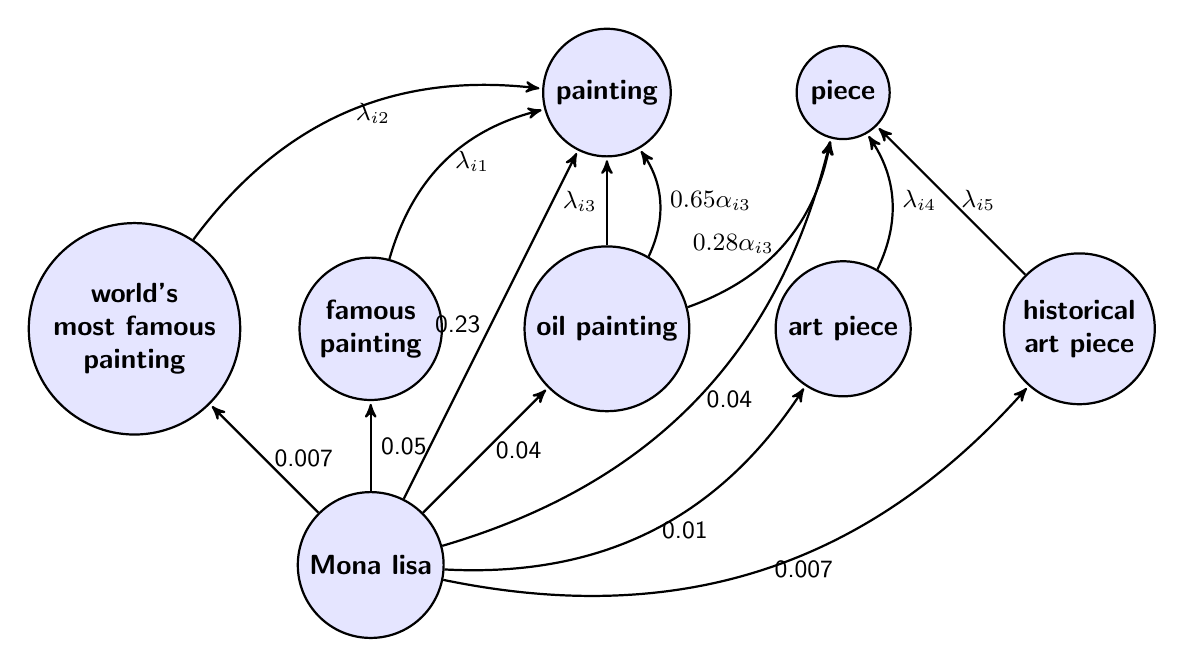
\begin{tikzpicture}[->,>=stealth',shorten >=1pt,auto,node distance= 3 cm,
  thick,main node/.style={circle,fill=blue!10,draw,font=\sffamily\bfseries,align = center}]

  \node[main node] (4) {piece};
  \node[main node] (2) [left of=4] {painting};

  \node[main node] (5) [below of=2] {oil painting};
  \node[main node] (6) [left of=5] {famous\\painting};
  \node[main node] (7) [left of=6] {world's\\most famous\\painting};

  \node[main node] (10) [right of=5] {art piece};
  \node[main node] (11) [right of=10] {historical\\art piece};

  \node[main node] (12) [below of=6] {Mona lisa};


  \path[every node/.style={font=\sffamily\small}]

    (5) edge  node [left] {$\lambda_{i3}$} (2)
        edge [bend right] node [right] {\small{$ 0.65\alpha_{i3} $}} (2)
        edge  [bend right] node[left]  {\small{$ 0.28\alpha_{i3} $}} (4)
    (6) edge [bend left] node [right] {$\lambda_{i1}$} (2)
    (7) edge [bend left] node [right] {$\lambda_{i2}$} (2)

    (10) edge [bend right] node[right] {$\lambda_{i4}$} (4)
    (11) edge node[right] {$\lambda_{i5}$} (4)
    (12) edge [bend right]node[right] {0.01} (10)
         edge [bend right]node[right] {0.007} (11)
         edge node[right] {0.04} (5)
         edge node[right] {0.05} (6)
         edge node[right] {0.007} (7)
         edge node[left] {0.23} (2)
         edge [bend right]node[right] {0.04} (4);

\end{tikzpicture}
\caption{calculating $P(\gamma_i|\term{Mona Lisa})$ }
\end{figure*}

The process of calculation is illustrated in the example~\ref{exa:calc}

\begin{example}[Calculating $P(\gamma_i|e)$]
\label{exa:calc}
As illustrated in Fig.~\ref{fig:pgge}, the process of calculating the typicality a concept is as follows, where \term{painting} is $\gamma_i$ and \term{Mona Lisa} is $e$. Then $P(\term{painting}|\term{Mona Lisa})$ consists of 2 parts, the direct edge $P_{original}(\gamma_i|e)= 0.23$, and the second part
$$\sum_{ c_{long}^*\in C_{long} } [ \lambda_{i}^*+(\alpha_{i}^*) P(\gamma_i|c_{long}^*) ] \times  P(c_{long}^*|e) $$
$(\alpha_i^*+\gamma_i^*=1)$
Thus we get
$$ P = 0.007\times \lambda_{i2}+0.05\times \lambda_{i1}+0.04\times(\lambda_{i3}+0.65\alpha_{i3}) $$
For \term{piece}, it is the similar process. The relation here is only part of the whole graph.
\end{example}




We consider only 2 layers of isA relationship for 2 reasons. The first one is that more layers will lead to noisy concepts such as \term{issue, factor, element}, which are concepts for almost eveything, Secondly, discussing the transitive relation between concepts is beyond the scope of this paper.


\section{Find Alias For Attributes}

For a pair \term{(Sherlock holmes, United Kindom)}, \term{country} is a merely-ok attribute, on the contrary, \term{residence, deathPlace} are better since they are more specific and more seemingly plausible to be an attribute.We argue that for each pair of entity, there is a selectional preference for attribute.

\nop{
Depending on the domain and range of the attribute , we can conceptualize
}
\subsection{Problem Definition}
Given a set of concept pairs ($\gamma_1$,$\gamma_2$), where $\gamma_1\in C_1$ and $\gamma_2\in C_2$, we want to find a set of attributes A, where for each $a \in A$:
we can form a ($\gamma_1$,$a$,$\gamma_2$) pair which best describe the relationship between $\gamma_1$ and $\gamma_2$.


\begin{figure}[!htb]
\centering 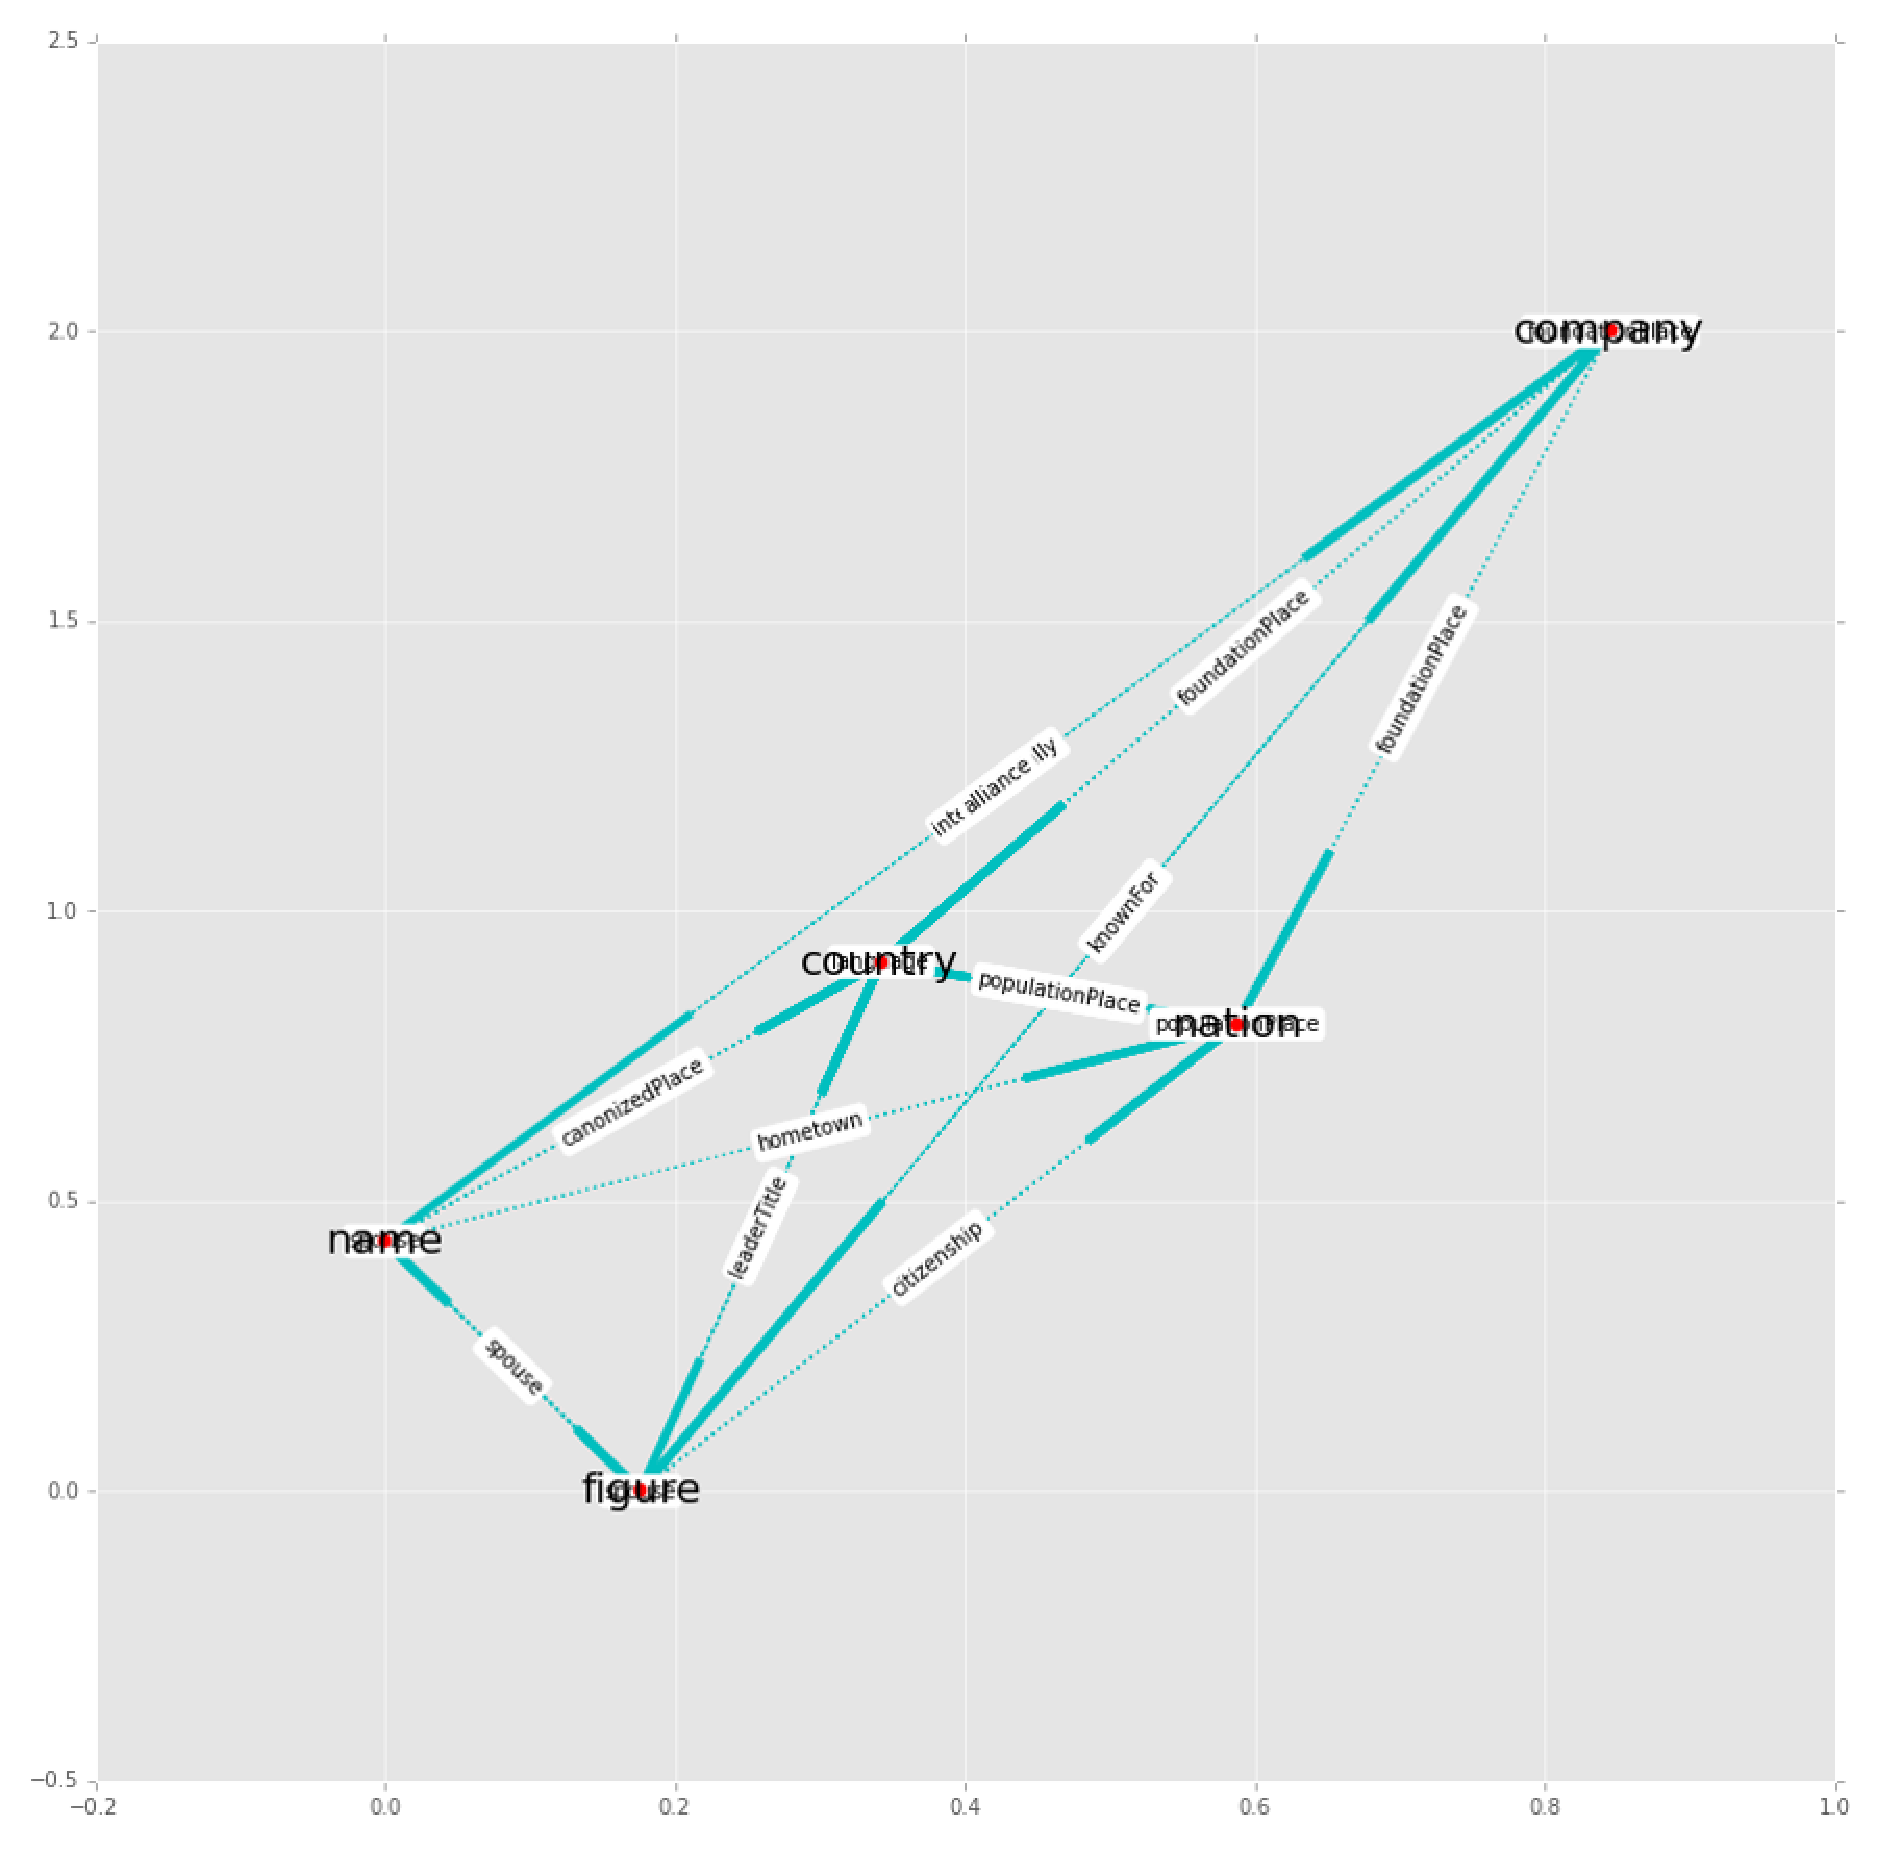
\epsfig{file=resources/eag.eps,width=2.5in}
\caption{Subgraph of Entity Attribute Graph } \label{fig:eag}
\end{figure}


\subsection{Problem Solution}

\subsubsection{Entity Attribute Graph Construction}

For any $(entity_1, attribute, entity_2)$ tuple, later denoted as  $(e_1, a, e_2)$ , where $e_1$ and $e_2$ are also referred to as \term{domain} and \term{range} of the attribute. We can conceptualize $e_1$ and $e_2$ using the method in section~\ref{sec:conceptualization}, and get a set of concept $C_1,C_2$, accompanied with a set of probabilities $P(\gamma_{1}|e_{1i})$, $P(\gamma_{2}|e_2)$,where ${\gamma_{1} \in C_1},{\gamma_{2} \in C_2}$.

To construct the Entity Attribute Graph, we only need topK concepts to form $(\gamma_1,\gamma_2)$ pair, K trough case study is around 5, so we here set K=10.

Thus for any attribute $a$, given a pair of entity $(e_{1i},e_{2j})$, we can define:
\xch{should i use joint ratio here?}

\begin{equation} \begin{split} P_{(e_{1i},e_{2j})}((\gamma_{1},\gamma_{2}) |a)&=P_{before}(\gamma_1|a) \times P_{after}(\gamma_2|a) \\&=  P(\gamma_{1}|e_{1i}) P(e_{1i}|a) \times P(\gamma_{2}|e_{2j})P(e_{2j}|a) \end{split} \label{eq:giga}\end{equation}


where we use $P_{(e_{1i},e_{2j})}((\gamma_{1},\gamma_{2}) |a)$ to denote observing a single pair $(e_{1i},e_{2j})$, how likely is a combination of $(\gamma_{1},a,\gamma_{2})$ to occur.

Consequently,
\begin{equation} P((\gamma_{1},\gamma_{2}) |a)=\sum_{  e_{1i} \in E_1 ,e_{2j} \in E_2} P_{(e_{1i},e_{2j})}((\gamma_{1},\gamma_{2}) |a) \label{eq:pg1g2ga}\end{equation}

where $E_1,E_2$ denoting the whole set of domain entity and range entity,The  $P(e_{1i}|a)$ and $P(e_{2j}|a)$ here has only 2 values $1$ and  $0$, depending on whether  $e_1$ occurs before $a$ or $e_2$ occurs after $a$. Apparently, only $(e_{1i}, a, e_{2j})$ occurs will give the equation a non-zero value, therefore, Eq.~\ref{eq:pg1g2ga} is finally equal to Eq.~\ref{eq:gga_fin}.

\begin{equation} \begin{split} P((\gamma_{1},\gamma_{2}) |a) &= \sum_{  (e_{1i},a,e_{2j})\in KB } P_{(e_{1i},e_{2j})}((\gamma_{1},\gamma_{2}) |a) \\&=  \sum_{  (e_{1i},a,e_{2j})\in KB }P(\gamma_{1}|e_{1i}) \times P(\gamma_{2}|e_{2j})\end{split} \label{eq:gga_fin}\end{equation}

\xch{
The process of calculating \term{} is demonstrated in Example.~\ref{exa:pggga}
}

\begin{example}[Calculating $P((\gamma_{1},\gamma_{2}) |a)$]
\label{exa:pggga}
As illustrated in Fig.~\ref{fig:bipartite}, the process of calculating $P((\gamma_{1},\gamma_{2}) |a)$ is as follows\term{}
\end{example}


\xch{insert a graph}
\begin{figure}[!htb]
\centering 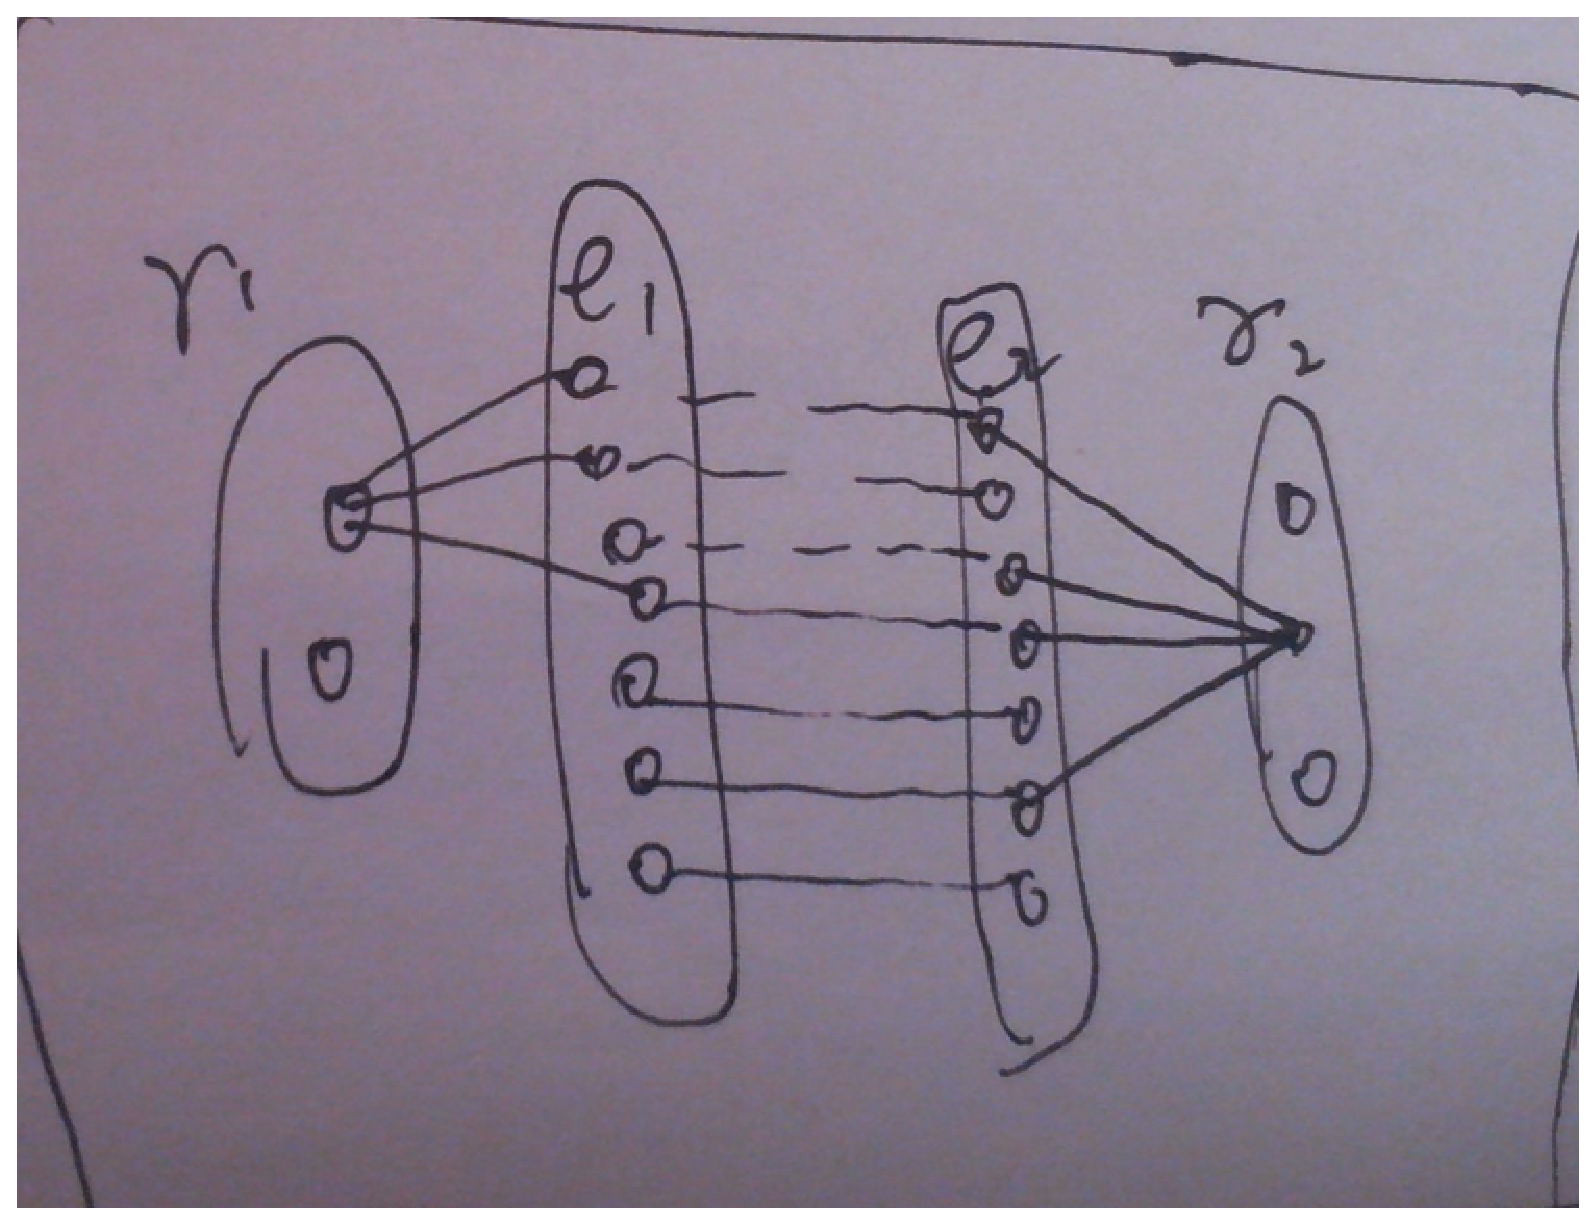
\epsfig{file=resources/bipartite.eps,width=2.5in}
\caption{Calculating $P((\gamma_{1},\gamma_{2}) |a$ for \term{}} \label{fig:bipartite}
\end{figure}

To Construct the Entity Attribute Graph, we calculate $P((\gamma_{1},\gamma_{2}) |a)$ for each attribute.




Note that we only consider the attributes whose range is an entity, and ignore those numerical values or date-and-time values such as $( Mona Lisa, Year, 1503)$.





For each $(\gamma_{1},a,\gamma_{2})$ tuple, we can calculate $P((\gamma_{1},\gamma_{2}) |a)$ for each







%\subsubsection{Voting}

\subsection{Find the best alias}

We then Use an $\argmax$ model to solve the problem.

Given $(e_1,e_2)$, our goal is to find the best attribute for it. We denote it as:
$$\argmax P((e_1,e_2)|a)$$







\section{Experiment}

\subsection{Head Concept Vs Original Concept}

\subsection{Find alias}
\subsubsection{compare}

Compare $ P((\gamma_{1i},\gamma_{2i} |a ))P(\gamma_{1i}|a) \times P(\gamma_{2i}|a)$




\subsubsection{Sense Disambiguation}

We can solve the problem of sense disambiguation problem well by applying this method since there are many entities belongs to the same concept and we only consider topK $(\gamma_1,\gamma_2)$ pairs that has high typicality $P( (\gamma_1,\gamma_2) |a)$, so that the weird $(\gamma_1,\gamma_2)$ patterns as manifest in Example.~\ref{exa:sd} can be easily filtered. 

\xch{cut the figure smaller}

\begin{figure}[!htb]
\centering 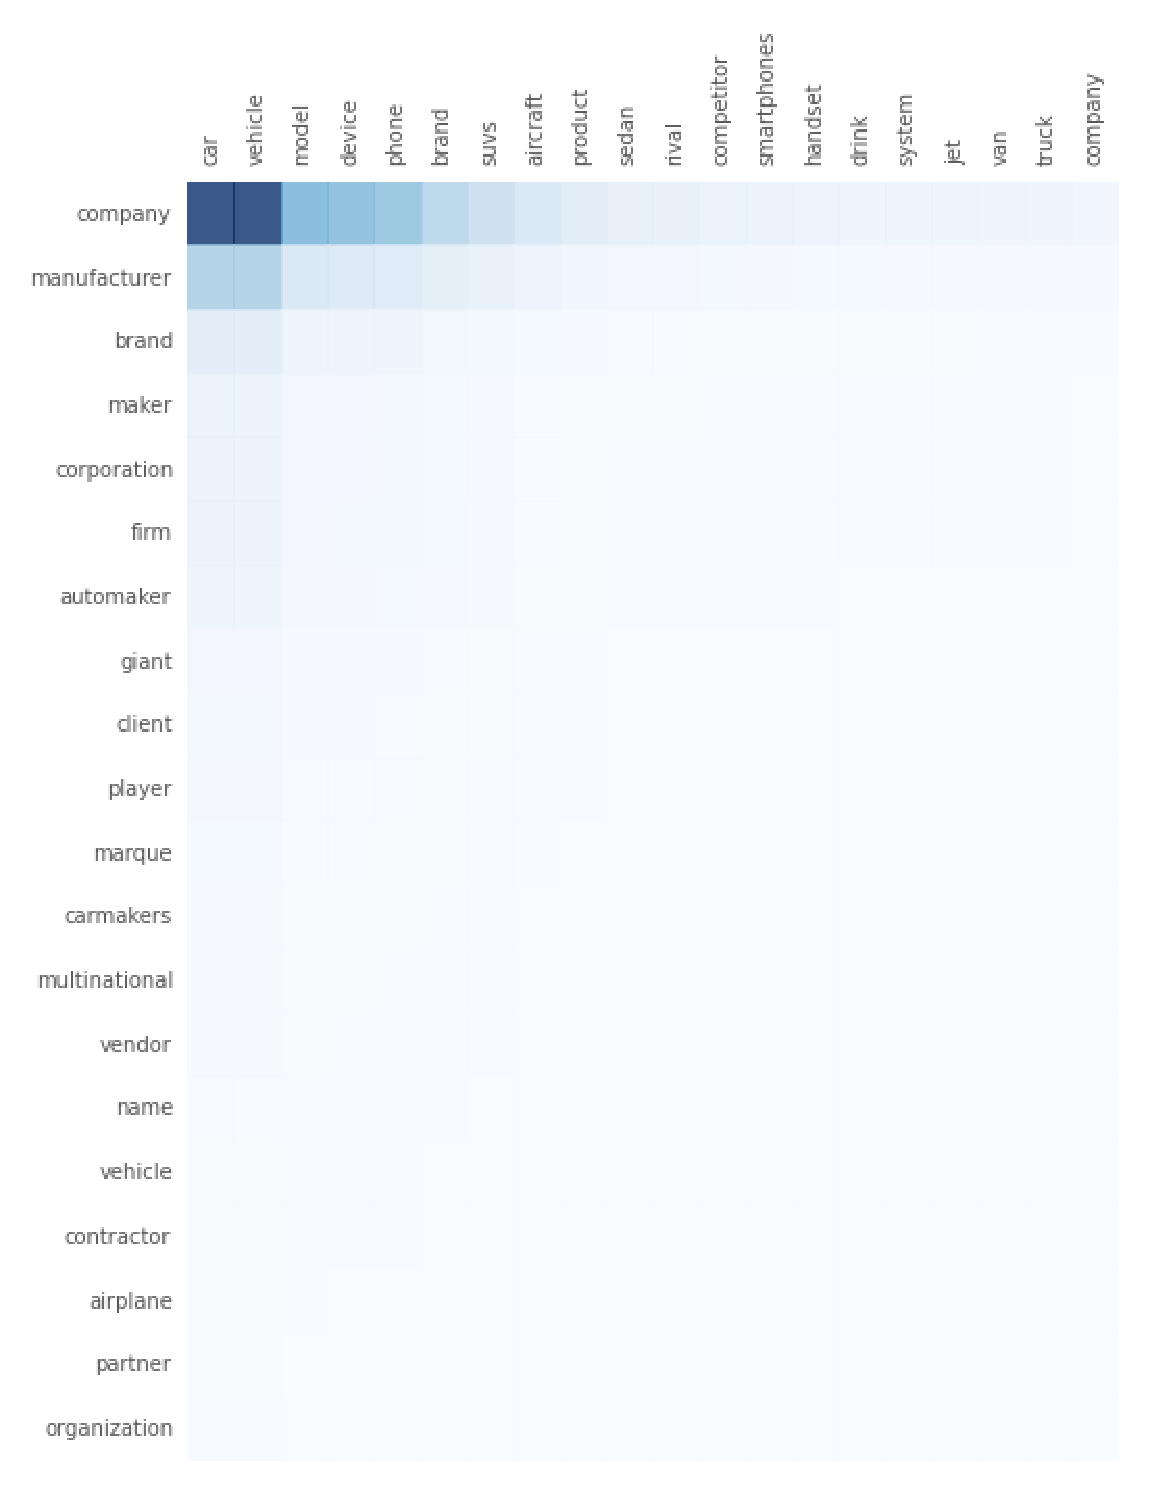
\epsfig{file=resources/ev_plot_manufacturer.eps,width=2.5in}
\caption{$(\gamma_1,\gamma_2$) plot for attribute \term{Manufacturer}} \label{fig:evplot}
\end{figure}

\begin{example}[Sense Disambiguation]
Consider the following $(e1,a,e2)$ tuple \term{(iphone, manufacturer, apple)}. Suppose it is our query, where \term{apple}'s sense can either be a kind of \term{fruit} or a \term{company}.
Fig.~\ref{fig:evplot} is a heatmap for all the concepts pairs $(\gamma_1,\gamma_2)$ of attributes \term{manufacturer}. The horizontal axis represents the $e_1$ and the vertical axis stands for $e_2$. The darker the blue is, the higher typicality it will be. In Fig.~\ref{fig:evplot}, We can observe that the top concepts of $e_2$ in the heatmap are \term{company, manufacturer,...} and top 10 pairs also does not include \term{fruit}. The intuition for this is that there exists thousands of $(e1,a,e2)$ tuple such as \term{(BMW\_Z4,manufacturer,BMW),(PlayStation\_4,manufacturer,Sony)} other than \term{(iphone, manufacturer, apple)} tuple, which results in a reasonable distribution.
\label{exa:sd}
\end{example}


\subsection{Selectional Preference}

\subsection{Evaluation}

\section{Conclusion}

\bibliographystyle{abbrv}
\bibliography{refer}

\end{document}